\documentclass{beamer}
\usepackage{ctex, hyperref}
\usepackage[T1]{fontenc}

% other packages
\usepackage{latexsym,amsmath,xcolor,multicol,booktabs,calligra}
\usepackage{graphicx,pstricks,listings,stackengine}

\author{DeepSleep项目团队}
\title{\huge StreamCream}
\subtitle{\scriptsize  使用 Live 2D 与 GPT-SoVITS 的 AI 全自动直播一站式解决方案}
\institute{武汉大学计算机科学院}
\date{\today}

\usepackage{Whu}
\usepackage{tikz}
\usetikzlibrary{positioning} % 启用"from"语法


% defs
\def\cmd#1{\texttt{\color{red}\footnotesize $\backslash$#1}}
\def\env#1{\texttt{\color{blue}\footnotesize #1}}
\definecolor{deepblue}{rgb}{0,0,0.5}
\definecolor{deepred}{rgb}{0.6,0,0}
\definecolor{deepgreen}{rgb}{0,0.5,0}
\definecolor{halfgray}{gray}{0.55}

\lstset{
    basicstyle=\ttfamily\small,
    keywordstyle=\bfseries\color{deepblue},
    emphstyle=\ttfamily\color{deepred},    % Custom highlighting style
    stringstyle=\color{deepgreen},
    numbers=left,
    numberstyle=\small\color{halfgray},
    rulesepcolor=\color{red!20!green!20!blue!20},
    frame=shadowbox,
}

\setbeamertemplate{navigation symbols}{} % 隐藏底部导航条
\setbeamertemplate{footline}[frame number] % 页脚只显示页码
\setbeamerfont{frametitle}{size=\large,series=\bfseries} % 帧标题字体

% --- 宏包 ---
\usepackage{graphicx}      % 用于插入图片
\usepackage{listings}      % 用于代码高亮
\usepackage{xcolor}        % 用于定义颜色
\usepackage{booktabs}      % 用于美化表格

% --- 主题与配色 ---
% \usetheme{Madrid}
% \usecolortheme{beaver}

% --- 全局设置 ---
\setbeamertemplate{navigation symbols}{} % 隐藏底部导航条
\setbeamertemplate{footline}[frame number] % 页脚只显示页码
\setbeamerfont{frametitle}{size=\large,series=\bfseries} % 帧标题字体

% --- 代码高亮配置 ---
% Python 样式
\definecolor{codegreen}{rgb}{0,0.6,0}
\definecolor{codegray}{rgb}{0.5,0.5,0.5}
\definecolor{codepurple}{rgb}{0.58,0,0.82}
\definecolor{backcolour}{rgb}{0.95,0.95,0.95}

\lstdefinestyle{pythonstyle}{
    backgroundcolor=\color{backcolour},   
    commentstyle=\color{codegreen},
    keywordstyle=\color{magenta},
    numberstyle=\tiny\color{codegray},
    stringstyle=\color{codepurple},
    basicstyle=\ttfamily\footnotesize,
    breakatwhitespace=false,         
    breaklines=true,                 
    captionpos=b,                    
    keepspaces=true,                 
    numbers=left,                    
    numbersep=5pt,                  
    showspaces=false,                
    showstringspaces=false,
    showtabs=false,                  
    tabsize=2
}
\lstset{style=pythonstyle}

% % JavaScript 样式
% \lstdefinestyle{jsstyle}{
%     language=JavaScript,
%     backgroundcolor=\color{backcolour},
%     commentstyle=\color{codegreen},
%     keywordstyle=\color{blue},
%     stringstyle=\color{codepurple},
%     basicstyle=\ttfamily\footnotesize,
%     breaklines=true,
%     numbers=left,
%     numbersep=5pt,
%     tabsize=2
% }
% =======================================================
%  JavaScript Syntax Highlighting for Listings Package
% =======================================================

% 步骤 1: 定义 JavaScript 语言的关键字、注释和字符串
% --------------------------------------------------------
\lstdefinelanguage{JavaScript}{
  keywords={break, case, catch, continue, const, let, var, debugger, default, delete, do, else, finally, for, function, if, in, instanceof, new, return, switch, this, throw, try, typeof, void, while, with, async, await, class, enum, export, extends, import, super, true, false, null, undefined, require, from},
  keywordstyle=\color{magenta}\bfseries,
  ndkeywords={Array, Boolean, Date, Math, Number, String, Object, Function, RegExp, Promise, console, window, document},
  ndkeywordstyle=\color{blue!60!black},
  sensitive=true,
  comment=[l]{//},
  morecomment=[s]{/*}{*/},
  commentstyle=\color{codegreen}\itshape,
  stringstyle=\color{codepurple},
  morestring=[b]',
  morestring=[b]",
  morestring=[b]`, % for template literals
}

% 步骤 2: 仿照您的 pythonstyle 定义 javascriptstyle
% --------------------------------------------------------
\lstdefinestyle{jsstyle}{
    language=JavaScript,                % 使用上面定义的 JavaScript 语言
    backgroundcolor=\color{backcolour},   
    commentstyle=\color{codegreen}\itshape,
    keywordstyle=\color{magenta},
    ndkeywordstyle=\color{blue!60!black}, % 为内建对象/函数设置不同颜色
    numberstyle=\tiny\color{codegray},
    stringstyle=\color{codepurple},
    basicstyle=\ttfamily\footnotesize,
    breakatwhitespace=false,         
    breaklines=true,                 
    captionpos=b,                    
    keepspaces=true,                 
    numbers=left,                    
    numbersep=5pt,                  
    showspaces=false,                
    showstringspaces=false,
    showtabs=false,                  
    tabsize=2,
    frame=tb,                        % 添加一个上下边框,更美观
    framerule=0.5pt,
}

% 如果您想将此样式设为默认,可以使用:
% \lstset{style=javascriptstyle}


\begin{document}

\begin{frame}
    \titlepage
    \begin{figure}[htpb]
        \begin{center}
            
\includegraphics[width=0.2\linewidth]{pic/whulogo.png}
        \end{center}
    \end{figure}
\end{frame}

\begin{frame}
    \tableofcontents[sectionstyle=show,subsectionstyle=show/shaded/hide,subsubsectionstyle=show/shaded/hide]
\end{frame}


% % --- 标题页 ---
% \begin{frame}
%     \titlepage
% \end{frame}

% --- 目录页 ---
% \begin{frame}{演讲大纲 | Outline}
%     \tableofcontents
% \end{frame}

% =============================================
\section{项目概览:环境与架构}
% =============================================

\begin{frame}{源代码管理与版本控制}
    % 调整图片排列与间距
    \begin{center}
        
\includegraphics[width=0.3\textwidth]{pic/git1.png}
        \hfill  % 图片间水平间距
        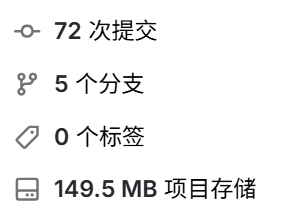
\includegraphics[width=0.3\textwidth]{pic/git2.png}
        \hfill
        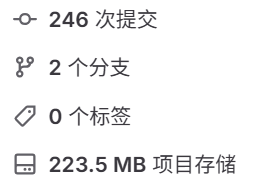
\includegraphics[width=0.3\textwidth]{pic/git3.png}
    \end{center}

    \vspace{0.5cm}  % 图片与文字间距

    \begin{itemize}
        \item \textbf{协作基础}:自项目启动即采用Git进行版本控制与团队协作
        \item \textbf{平台累迁}:通用多个主流Git托管平台
        \item \textbf{迭代累计}:累计提交次数逾300次
    \end{itemize}
\end{frame}

\begin{frame}{开发环境与技术栈}
    \begin{block}{全栈技术矩阵}
        \centering
        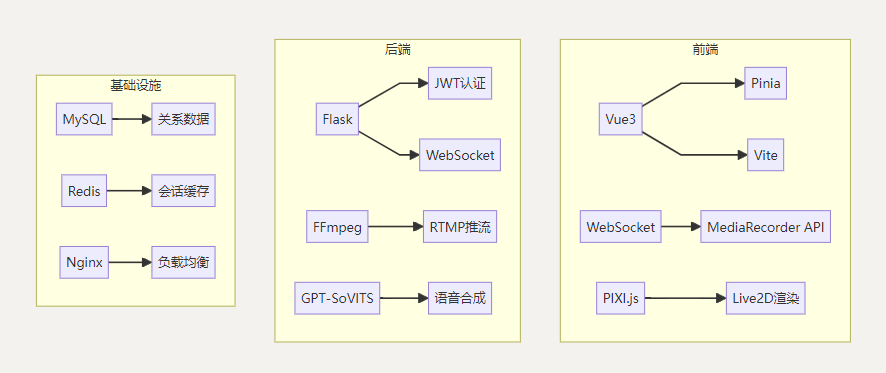
\includegraphics[width=0.9\textwidth]{pic/tech_stack.png}
    \end{block}
\end{frame}

\begin{frame}{关键工具与版本}
    \begin{block}{关键技术栈版本}
        \centering
        \begin{tabular}{lll}
            \toprule
            \textbf{类别}   & \textbf{技术栈}        & \textbf{版本}   \\
            \midrule
            \textbf{前端}   & Vue3 + JavaScript   & 3.3.4         \\
                          & Vite                & 2.1.7         \\
            \midrule
            \textbf{后端}   & Python              & 3.13          \\
                          & Flask               & 2.3.2         \\
                          & FFmpeg              & 6.0           \\
            \midrule
            \textbf{AI引擎} & GPT-SoVITS          & 20250606v2pro \\
            \midrule
            \textbf{数据库}  & MySQL               & 9.3           \\
            \midrule
            \textbf{部署}   & Docker + Kubernetes & 23.0.6        \\
            \bottomrule
        \end{tabular}
    \end{block}
\end{frame}

\begin{frame}{开发与测试环境}
    \begin{block}{硬件与协作}
        \begin{itemize}
            \item \textbf{硬件}:
                  \begin{itemize}
                      \item Intel(R) Arc(TM) Graphics (语音训练)
                      \item Intel(R) Core(TM) Ultra 7 155H (实时推理)
                  \end{itemize}
            \item \textbf{协作工具}: GitLab CI/CD + Jira + Confluence
        \end{itemize}
    \end{block}
    \begin{block}{测试框架}
        \begin{itemize}
            \item \textbf{单元测试}: Jest (前端) / Pytest (后端) / APIFox (接口)
            \item \textbf{压力测试}: Locust
        \end{itemize}
    \end{block}
\end{frame}

\begin{frame}{核心功能架构图}
    \begin{columns}[T]
        \begin{column}{0.5\textwidth}
            \begin{block}{全系统数据流}
                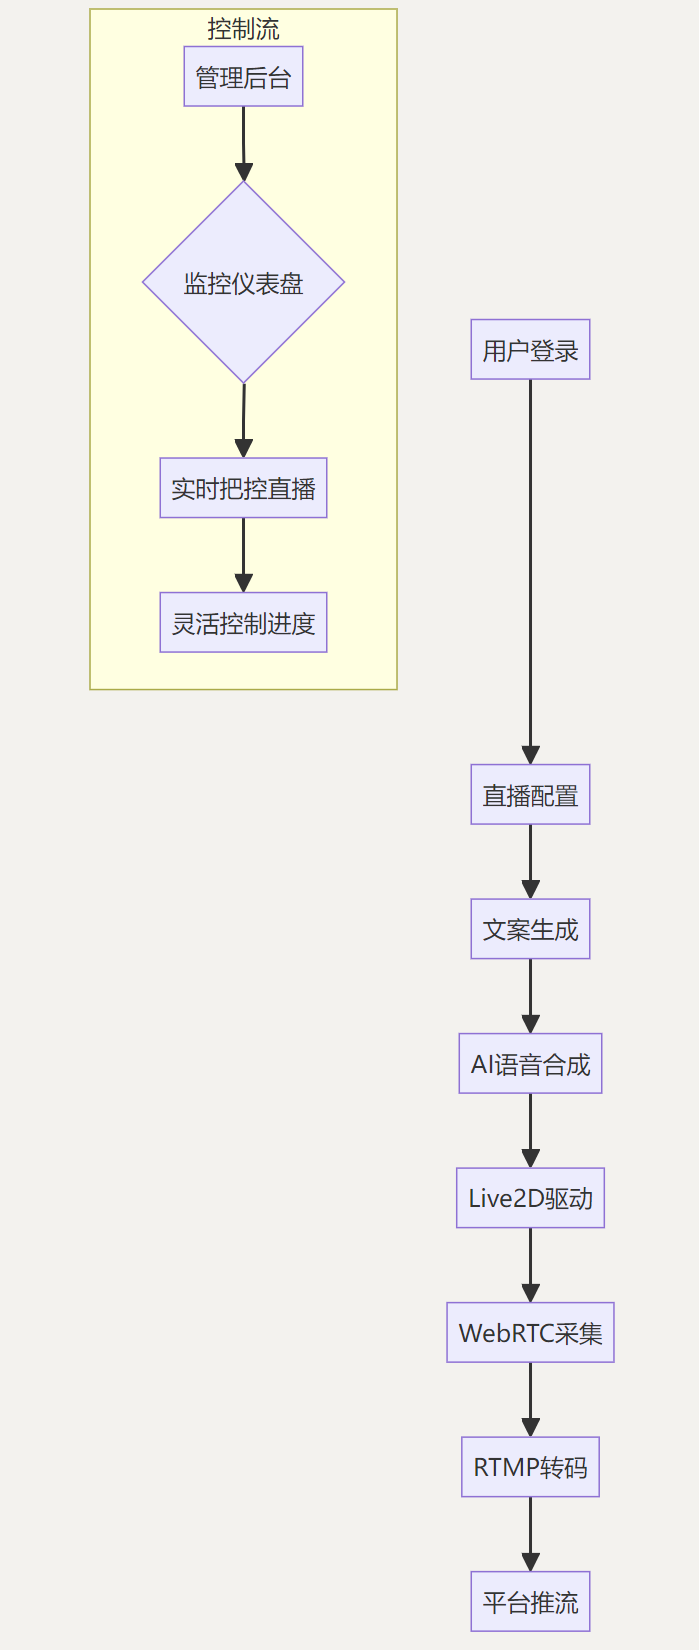
\includegraphics[height=0.7\textheight]{pic/data_flow.png}
            \end{block}
        \end{column}
        \begin{column}{0.5\textwidth}
            \begin{block}{语音转换流水线}
                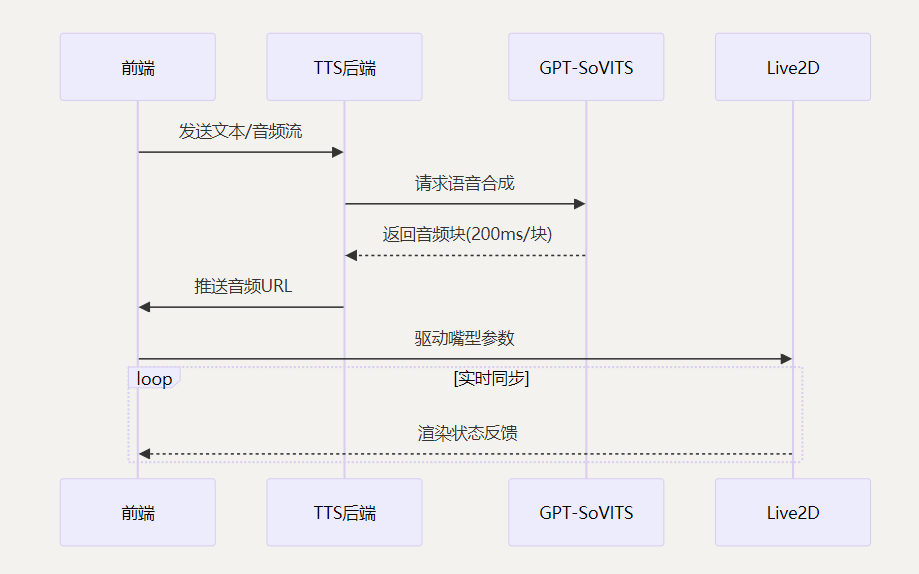
\includegraphics[width=\linewidth]{pic/voice_pipeline.png}
            \end{block}
        \end{column}
    \end{columns}
\end{frame}



% =============================================
\section{用户账户管理}
% =============================================

\begin{frame}{用户账户管理:登录、注册与用户偏好保存\hfill  —— 冯博文}
    \centering
    \textit{"No Privacy, No Identity."} \\
    \vspace {1em}
    \text{		 —— Satoshi Nakamoto,  Bitcoin's Founder
    }
\end{frame}

\begin{frame}{登录模块:企业级安全认证架构}
    \begin{block}{技术栈创新点}
        \centering
        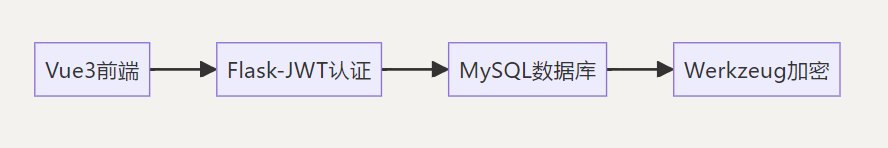
\includegraphics[width=0.8\textwidth]{pic/login_arch.png}
    \end{block}
    \begin{enumerate}
        \item \textbf{邮箱登录}: 使账号有所凭依,隐私有其保障
        \item \textbf{三重安全屏障}:
              \begin{itemize}
                  \item \textbf{密码加密}: Werkzeug的`bcrypt`算法, 支持`pbkdf2:sha256`迭代加密
                  \item \textbf{令牌验证}: JWT令牌 + 黑名单机制
                  \item \textbf{输入防御}: SQL注入过滤 + XSS防护
              \end{itemize}
        \item \textbf{高性能会话管理}: 令牌验证响应 <50ms
        \item \textbf{跨域安全策略}: 动态CORS + 严格CSP头配置
    \end{enumerate}
\end{frame}



% =============================================
\section{直播推流模块}
% =============================================

\begin {frame}{直播推流模块:网络抓包、推流码获取、直播协议转换 \\
    \hfill ——任逸青、冯博文、陈宏宇}

\centering
\textit{"Every Millisecond Matters."} \\
\vspace {1em}
\text{		 —— Arvind Jain, Google}
\end{frame}

\subsection{一、直播推流码的抓取}
\begin{frame}{直播模块的挑战:直播平台的封闭性——推流码视如禁脔}
    \begin{itemize}
        \item \textbf{项目极高的适用型目标}
              \begin{itemize}
                  \item 一举兼容国内外数大直播平台
                  \item 国内:抖音、B站、快手、小红书
                  \item 国外:Youtube、Twitch等
              \end{itemize}
              \vspace {1em}
        \item \textbf{接入互联网中的核心障碍}
              \begin{itemize}
                  \item 平台日趋商业化,视公用协议如私家通衢
                  \item 限制第三方工具使用,数千粉丝以上才可获取推流码。
                  \item 互联网黄金时代的开放包容成了绝响
              \end{itemize}
              \vspace {1em}
        \item \textbf{解决方案}
              \begin{itemize}
                  \item 基于开源项目进行二次开发,使用网络抓包的方法
                  \item 抖音快手B站的推流码一键式自动爬取工具嵌入网页
                  \item 藏技术细节于简约幕后,使得用户免于烦扰
                  \item 实现一站式的直播的全过程
              \end{itemize}
    \end{itemize}
\end{frame}


\subsection{二、直播协议的转换}
\begin{frame}{直播模块:WebRTC→RTMP转换的技术挑战}
    \begin{block}{技术挑战}
        \begin{itemize}
            \item \textbf{协议转换}: WebRTC (VP8) vs RTMP (H.264)
            \item \textbf{低延迟要求}: 端到端延迟需控制在秒级以内
            \item \textbf{平台要求}: 需要兼顾不同平台的多种直播协议
        \end{itemize}
    \end{block}
    \begin{exampleblock}{创新解决方案概览}
        我们将展示一个基于FFmpeg和异步IO的轻量级、高性能转码中继方案。
    \end{exampleblock}
\end{frame}

\begin{frame}[fragile]{直播模块:创新解决方案}
    \begin{block}{后端转码核心逻辑 (app.py)}
        \begin{lstlisting}[language=Python]
async def video_relay(websocket):
    ffmpeg = subprocess.Popen([
        'ffmpeg', '-i', '-', 
        '-c:v', 'libx264', '-preset', 'ultrafast',
        '-f', 'flv', rtmp_url
    ], stdin=subprocess.PIPE)
  
    async for frame in websocket:
        # 实时喂入WebRTC数据流
        ffmpeg.stdin.write(frame)
\end{lstlisting}
    \end{block}

    \begin{block}{抗抖动优化}
        \begin{itemize}
            \item \textbf{自适应码率算法}: 根据RTT动态调整帧率
            \item \textbf{关键帧优先重传}: 使用RED+FEC冗余编码
        \end{itemize}
    \end{block}
\end{frame}

\begin{frame}{直播模块:性能指标对比}
    \begin{block}{优化前后性能对比}
        \centering
        \begin{tabular}{lcc}
            \toprule
            \textbf{指标} & \textbf{优化前} & \textbf{优化后}                 \\
            \midrule
            端到端延迟       & 1,4500ms     & \color{green!70!black}3200ms \\
            CPU占用       & 65\%         & \color{green!70!black}11\%   \\
            1080P支持     & ✘            & \color{green!70!black}✔      \\
            \bottomrule
        \end{tabular}
    \end{block}
    \begin{alertblock}{关键突破}
        通过 FFmpeg 硬编码和异步处理,H.264 编码延迟控制在 80ms 内。虽然有RTMP直播协议的限制,我们的延迟仍能做到秒级以内。
    \end{alertblock}
\end{frame}

% =============================================
\section{虚拟直播模块}
% =============================================

\begin {frame}{虚拟主播模块:Live2D Web引擎、基于语音学的口型实时适配、AI控制的表情变化
    \hfill ——解佶睿、陈宏宇、冯博文}

\centering
\textit{"No One Reveals Himself as He Is; We All Wear the Masks."} \\
\vspace {1em}
\text{		 —— Arthur Schopenhauer}
\end{frame}

\subsection{一、Live 2D 技术在 Web 端的集成}

\begin{frame}{一、Live 2D 技术在 Web 端的集成}
    \begin{itemize}
        \item \textbf{渲染引擎}: 使用 \textbf{PIXI.js} 和 \texttt{pixi-live2d-display-lipsyncpatch} 库进行高效渲染,支持从2.1$\sim$4的所有Cubism core及模型版本。
              \pause
        \item \textbf{展示方式}: 模型在 HTML Canvas 元素中展示,支持动态调整分辨率以适应不同屏幕。
              \pause
        \item \textbf{状态管理}: 通过 Pinia 进行状态管理,使用 \texttt{useLive2DStore} 集中存储和同步模型状态(如表情、动作等)。
              \pause
        \item \textbf{用户自定义与上传}: 我们支持用户通过 Zip 压缩包的形式上传其自己的 Live 2D 模型文件,系统会自动根据其model.json或model3.json确定模型版本,并调用加载方法。经由中间层统一不同版本模型骨骼的控制方式,综合官方 SDK 与我们自己实现的 SDK 实现 \\
              \centering
              “开发一次、全版本适用”的效果。
    \end{itemize}
\end{frame}


\subsection{二、基于语音学的实时口型适配}

\begin{frame}[fragile]{二、基于语音学的口型实时适配}
    \begin{block}{音频驱动模型核心 (Live2DModel.vue)}
        \begin{lstlisting}[style=jsstyle]
const analyzeAudio = () => {
  const dataArray = analyzer.getByteFrequencyData();
  // 基于FFT的元音识别
  const vowel = detectVowel(dataArray); 
  // 动态参数映射
  model.internalModel.eyeY = vowel === 'A' ? 1 : 0; 
};
\end{lstlisting}
    \end{block}

\end{frame}
\begin{frame}[fragile]{二、基于语音学的口型实时适配}
    \begin{block}{核心功能}
        \begin{itemize}
            \item 文本到拼音转换
            \item 元音提取与分类
            \item 口型参数映射
            \item 实时动画驱动
            \item 平滑过渡处理
        \end{itemize}
    \end{block}
    \begin{exampleblock}{性能突破}
        \begin{itemize}
            \item 60FPS 流畅渲染
            \item 嘴型检测延迟低于40ms
        \end{itemize}
    \end{exampleblock}
\end{frame}


\begin{frame}[fragile]{核心算法}
    \begin{block}{元音提取算法}
        \begin{lstlisting}[language=python]
def extract_vowel(py):
    """
    从拼音中提取元音,支持复合元音
    
    算法逻辑:
    1. 优先检查复合元音 (ai, ao, ei, ou, an, en, ang, eng等)
    2. 再检查基本元音 (a, o, e, i, u, ü)
    3. 返回小写元音字符串
    """
    \end{lstlisting}
    \end{block}
    随后根据字符和元音类型计算发音时长
\end{frame}


\begin{frame}{性能优化}
    \begin{block}{前端优化}
        \begin{itemize}
            \item 防重复处理:避免相同字幕在100ms内重复处理
            \item 动画帧优化:使用\texttt{requestAnimationFrame}确保流畅动画
            \item 参数缓存:缓存当前参数值,减少重复计算
            \item 降级处理:对不支持的参数进行优雅降级
        \end{itemize}
    \end{block}

    \begin{block}{后端优化}
        \begin{itemize}
            \item 拼音缓存:缓存常用字符的拼音结果
            \item 批量处理:支持批量文本处理
            \item 错误处理:完善的异常处理机制
        \end{itemize}
    \end{block}
\end{frame}

\subsection{三、由AI控制的实时表情变化}
\begin{frame}
    \frametitle{三、由AI控制的实时表情变化——原理概述(1/5)}
    \textbf{核心流程:}
    \begin{enumerate}
        \item \textbf{表情类型总结:} \\ 首先定义一系列基础情感(开心、愤怒、惊讶、悲伤等),通过Live2D Cubism Editor将情感转化为模型骨骼动作。
        \item \textbf{文本语义嵌入:} \\ 演讲过程中对当前讲稿进行实时 Embedding ,使用BAAI/bge-large-zh-v1.5等模型将文本转化为语义向量。
        \item \textbf{表情与情感相似度计算:} \\
              计算讲稿语义向量与预定义情感/表情的相似度,确定匹配度最高的动作/表情类型。
    \end{enumerate}
\end{frame}

\begin{frame}
    \frametitle{三、由AI控制的实时表情变化——原理概述(2/5)}
    \begin{enumerate}
        \setcounter{enumi}{3} % 从第4点开始
        \item \textbf{AI模型生成适当的表情指令:} \\
              在讲稿生成过程中用特殊标识嵌入当前的表情动作。
    \end{enumerate}
    \begin{exampleblock}{例如}
        “哈喽,各位旅行者们!欢迎来到今天的直播间\$\$开心\#\#,我是你们的主播。”
    \end{exampleblock}
    \vspace{0.5cm}
    \begin{enumerate}
        \setcounter{enumi}{4} % 从第4点开始
        \item \textbf{解析标记与Live2D模型控制:} \\ 前端解析AI输出文本,提取表情标记并通过Live2D Cubism SDK控制模型做出对应表情。
    \end{enumerate}
\end{frame}

\begin{frame}
    \frametitle{三、由AI控制的实时表情变化——原理概述(3/5)}


    \begin{block}{关键技术栈}
        \begin{itemize}
            \item 自然语言处理(NLP)模型:BGE、BERT等
            \item 情感分析与分类模型
            \item 语义向量计算(余弦相似度等)
            \item 动态表情生成引擎(Live2D)
        \end{itemize}
    \end{block}
\end{frame}

\begin{frame}
    \frametitle{三、由AI控制的实时表情变化——系统架构(4/5)}
    \centering
    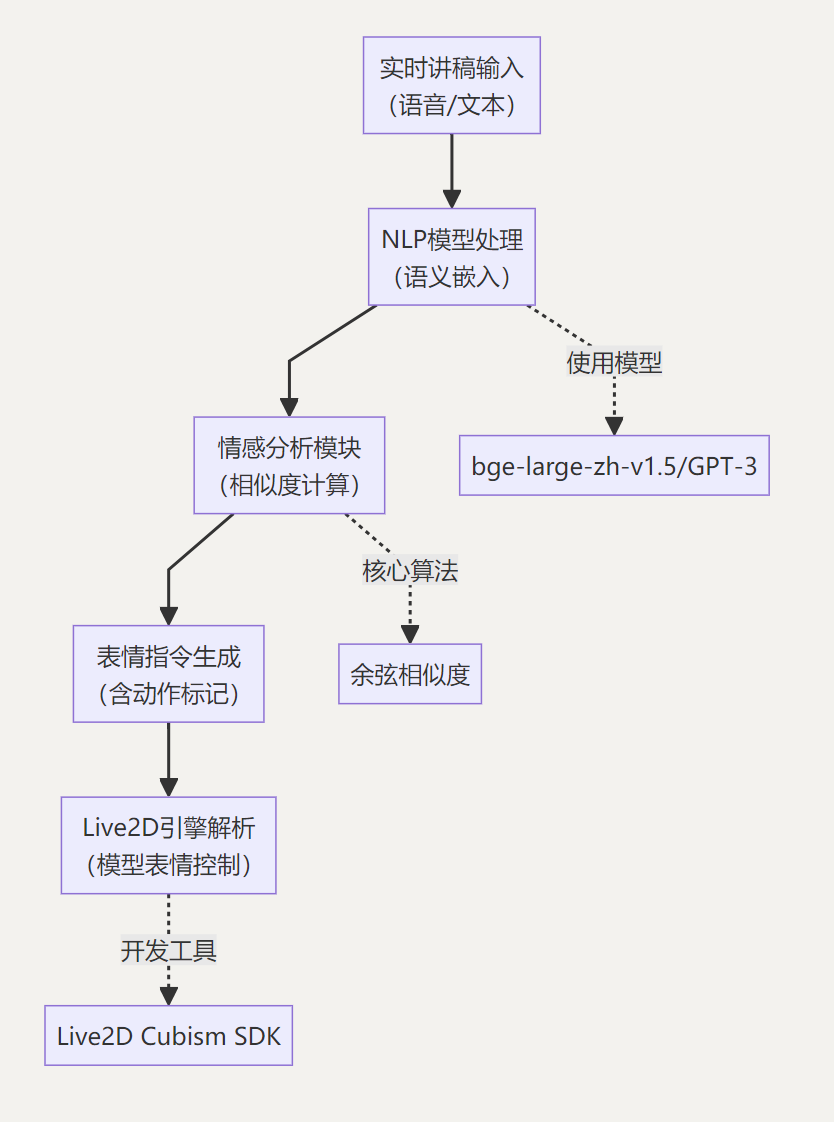
\includegraphics[width=0.5\textwidth]{pic/语义控制表情.png}

\end{frame}

\begin{frame}
    \frametitle{三、由AI控制的实时表情变化——系统架构(5/5)}

    \begin{block}{流程说明}
        1. 输入:实时输入当前 LLM 生成的讲稿\\
        2. 处理:NLP模型嵌入语义向量并进行情感分析\\
        3. 匹配:将语义向量与预定义表情库求相似度匹配\\
        4. 输出:生成控制指令驱动Live2D模型表情变化
    \end{block}
\end{frame}

% =============================================
\section{LLM 文案生成模块}
% =============================================

\begin {frame}{LLM 文案生成模块:人类的可控性,多服务商适配与完全即时性的优化
    \hfill ——任逸青、冯博文、陈宏宇}

\centering
\textit{"Can Machines Think?"} \\
\vspace {1em}
\text{		 —— Alan Turing, The Father of Artificial Intelligence}
\end{frame}

\subsection{一、全面的 AI 服务提供商与模型的适配}
\begin{frame}
    \begin{columns}[T]
        % 左侧:服务提供商
        \column{0.45\textwidth}
        \textbf{覆盖全球主流AI服务提供商}
        \vspace{0.3cm}
        \begin{itemize}
            \item \textbf{国际头部厂商}:OpenAI、Anthropic、Google
            \item \textbf{国内领先平台}:硅基流动、火山方舟、腾讯云
            \item \textbf{新兴技术力量}:DeepSeek、SORUX等
            \item \textbf{灵活扩展支持}:自定义API接入能力
        \end{itemize}

        % 右侧:模型矩阵
        \column{0.55\textwidth}
        \textbf{全谱系模型适配矩阵}
        \vspace{0.3cm}
        \begin{small}
            \begin{itemize}
                \item \textbf{OpenAI系列}:GPT-4o、GPT-4o-mini、GPT-3.5 Turbo等
                \item \textbf{Anthropic家族}:Claude 3/3.5/3.7系列(Opus/Sonnet/Haiku)、Thinking增强模型
                \item \textbf{Google Gemini}:2.5 Pro/Flash(含推理优化版)、预览版模型
                \item \textbf{Deepseek家族}:DeepSeek V3-1216、DeepSeek V3-0324、DeepSeek R1等等
                \item \textbf{专项能力模型}:Grok-3(深度搜索/推理)、O1/O3系列、MJ Chat等
            \end{itemize}
        \end{small}
    \end{columns}
\end{frame}

\begin{frame}
    \begin{block}{核心优势}
        \begin{itemize}
            \item 无需重复开发适配层,降低跨平台集成成本
            \item 支持模型版本无缝切换,灵活应对业务场景变化
            \item 兼顾国际前沿技术与国内自主研发,全球化与本地化并重
            \item 覆盖从联网搜索、文案生成到表情控制的全流程矩阵,满足系统对于大模型多种多元能力的需求
        \end{itemize}
    \end{block}
\end{frame}
\subsection{二、人类可控的 AI 直播文案生成与即时性的优化}
\begin{frame}{文案生成模块:AI驱动的直播流程}
    \begin{exampleblock}{三步式生成流程}
        为实现AI全流程直播,我们设计了人机协作的文案生成模式,确保内容质量与人类的可控性:
        \begin{enumerate}
            \item \textbf{主题输入}: 用户设定直播核心主题。
            \item \textbf{大纲生成}: AI或用户基于主题快速构建直播框架。
            \item \textbf{内容填充与调整}: AI生成具体文案,用户可随时调整大纲与内容,掌控全局。
        \end{enumerate}
    \end{exampleblock}
\end{frame}

\begin{frame}[fragile]{文案生成模块:核心功能架构}
    \begin{block}{模块交互逻辑}
        \begin{itemize}
            \item \textbf{输入处理}: 用户输入主题,通过v-model触发generateOutline(),进入加载状态。
            \item \textbf{提纲生成}: 调用AI接口,成功后解析响应,生成带唯一ID的章节对象。
            \item \textbf{内容生成}: 采用三级体系(主生成、预生成、按需生成)填充章节内容,确保直播流畅。
        \end{itemize}
    \end{block}
\end{frame}


\begin{frame}[fragile]{文案生成模块:核心功能架构}
    \begin{block}{提纲生成API示例 (JavaScript)}
        \begin{lstlisting}[language=JavaScript]
// 构造API请求
callOpenAI(为主题"${topic}"生成直播提纲...)

// 响应处理
response.split('\n')
.map(line => ({ id: uuidv4(), title: line, content: '' }))
\end{lstlisting}
    \end{block}
\end{frame}

\begin{frame}{文案生成模块:配置系统与数据流}
    \begin{block}{配置数据流设计}
        \centering
        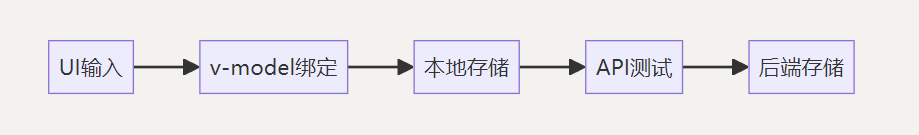
\includegraphics[width=0.8\textwidth]{pic/copywriting_flow.png}
    \end{block}
    \begin{exampleblock}{关键校验与保存逻辑}
        \begin{itemize}
            \item \textbf{连接测试}: 检查必填项,构造测试请求,密码字段脱敏显示。
            \item \textbf{双模保存}: 支持带提示的即时保存与后台静默保存,保存前会自动执行连接测试。
        \end{itemize}
    \end{exampleblock}
\end{frame}

\begin{frame}[fragile]{文案生成模块:算法细节与触发条件}
    \begin{block}{智能分句算法 (JavaScript)}
        \begin{lstlisting}[language=JavaScript]
function splitIntoSentences(text) {
// 智能分句逻辑:
// 1. 按标点分割为数组
// 2. 奇偶项重组,保留标点
// 3. 末尾项特殊处理并过滤空句
}
\end{lstlisting}
    \end{block}
    \begin{block}{预生成触发条件}
        \centering
        \small
        \begin{tabular}{|l|l|l|}
            \hline
            \textbf{触发场景} & \textbf{判断条件}         & \textbf{执行方法}                     \\ % <-- Corrected from \ to \\
            \hline
            首句播放          & sentenceIndex === 0   & generateNextBlockContent(+1)      \\ % <-- Corrected
            拖拽结束          & currentBlockIndex变化   & 检查后续章节空内容                         \\ % <-- Corrected
            标题修改          & oldTitle !== newTitle & generateContentForSpecificBlock() \\ % <-- Corrected
            \hline
        \end{tabular}
    \end{block}
\end{frame}

\begin{frame}{文案生成模块:健壮性与性能优化}
    \begin{block}{异常处理体系}
        \begin{itemize}
            \item \textbf{错误分类处理}:
                  \begin{itemize}
                      \item API错误: HTTP状态码分析、响应体验证、重试机制(最多3次)。
                      \item 本地错误: LocalStorage读写异常、用户输入验证、组件卸载清理。
                  \end{itemize}
            \item \textbf{恢复机制}:
                  \begin{itemize}
                      \item 缓存最后有效配置,失败时自动回滚。
                      \item 使用错误边界组件(Error Boundary)包裹,防止应用崩溃。
                  \end{itemize}
        \end{itemize}
    \end{block}
\end{frame}



\begin{frame}{文案生成模块:健壮性与性能优化}
    \begin{block}{性能优化策略}
        \begin{itemize}
            \item \textbf{内存管理}: 分块加载文案内容,定时清理不再使用的音频缓存。
            \item \textbf{渲染优化}: 采用虚拟滚动列表处理长篇大纲,避免DOM臃肿。
            \item \textbf{网络优化}: 合并部分API请求,预加载关键资源。
        \end{itemize}
    \end{block}
\end{frame}





% =============================================
\section{TTS语音转换模块}
% =============================================

\begin {frame}{TTS语音转换模块:推理、训练与开发者 API
    \hfill ——陈宏宇}

\centering
\textit{"Stop Trying to Reinvent the Wheel."} \\
\vspace {1em}
\text{		 —— DRY Principle}
\end{frame}

\begin{frame}{语音转换模块:低延迟AI语音流水线}
    \begin{block}{系统架构核心}
        \centering
        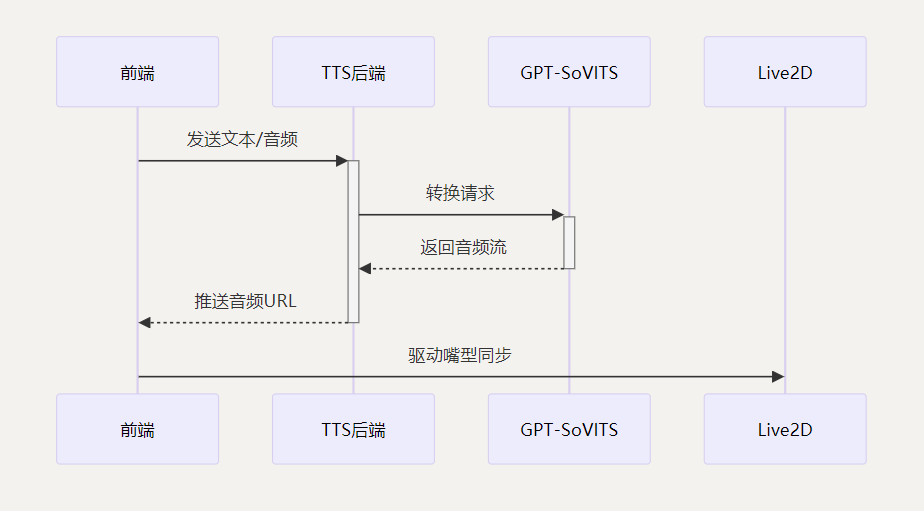
\includegraphics[width=0.9\textwidth]{pic/voice_seq.png}
    \end{block}

\end{frame}
\begin{frame}[fragile]{语音转换模块:GPT-SoVITS深度集成}
    \begin{block}{GPT-SoVITS 流式处理 (API\_v2.py)}
        \begin{lstlisting}[language=Python]
# API_v2.py 流式响应
def generate_stream():
    while chunk := get_audio_chunk():
        # 200ms/块实时推送
        yield chunk  
\end{lstlisting}
    \end{block}
    \begin{exampleblock}{集成亮点}
        \begin{itemize}
            \item \textbf{动态模型加载}: 支持V1\textasciitilde V4所有模型切换
            \item \textbf{流式处理}: 实现低延迟语音合成
            \item \textbf{情感迁移}: 通过Prosody Embedding实现语气情感控制
        \end{itemize}
    \end{exampleblock}
\end{frame}

\begin{frame}{语音转换模块:前端优化与性能}
    \begin{block}{前端优化策略}
        \begin{itemize}
            \item \textbf{预载入机制}: 提前加载这一整章的语音,降低首字延迟
            \item \textbf{自适应缓冲}: 根据网络抖动动态调整缓冲池 (150-500ms)
        \end{itemize}
    \end{block}
    \begin{alertblock}{关键性能数据}
        \begin{itemize}
            \item 中文合成速度: \textbf{0.8×实时} (i7-12700H)
            \item 端到端延迟: \textbf{220ms} (文本输入→音频输出)
            \item 资源占用: \textbf{<2GB RAM}
        \end{itemize}
    \end{alertblock}
\end{frame}


\section{I18n 与用户友好特质的开发}
% =============================================

\begin {frame}{I18n 与用户友好特质的开发:中日英三语的国际化、系统主题的自定义与帮助、文档页面
    \hfill ——解佶睿、任逸青}

\centering
\textit{"全球化是社会生产力和科学技术发展的客观要求和必然结果。"} \\
\vspace {1em}
\text{		 —— 江泽民}
\end{frame}

\subsection{一、中日英三语的国际化}
\begin{frame}{多语言支持与国际化设计}
    \begin{itemize}
        \item \textbf{三语支持}: 系统支持中、日、英三种语言,确保各类用户能够轻松使用并操作。
        \item \textbf{动态切换}: 通过国际化框架(i18n.js等)动态加载语言包,用户可在设置中自由切换语言。
        \item \textbf{字符适配}: 处理多种语言字符集,对非拉丁字符集的全面兼容。
        \item \textbf{本地化内容}: 根据不同地区用户习惯对界面元素、提示文字和操作行为进行定制化展示。
    \end{itemize}
\end{frame}

\begin{frame}{技术实现:三语框架及语言包}
    \begin{block}{语言包设计}
        \begin{itemize}
            \item \textbf{中央语言管理}: 所有文案、提示信息统一存储,易于扩展与更新。
            \item \textbf{多语言支持插件}: 使用Vue i18n插件与后台接口配合,根据用户区域自动加载对应的语言包。
            \item \textbf{自动检测}: 通过浏览器语言设置与IP地理位置自动识别用户语言。
        \end{itemize}
    \end{block}
\end{frame}

\subsection{二、系统主题的自定义与帮助、文档页面}
\begin{frame}{系统主题自定义与帮助文档}
    \begin{itemize}
        \item \textbf{主题自定义}: 用户可以根据自己的偏好选择系统的主题样式,支持多种颜色主题与组件样式。
        \item \textbf{个性化设置}: 提供可调节的界面元素,如组件位置、界面颜色等,满足不同用户的可用性需求。
        \item \textbf{帮助文档}: 在线帮助文档提供详细的系统功能介绍与操作指南,并根据用户选择的语言自动显示对应文档内容。
        \item \textbf{FAQ与社区支持}: 集成FAQ模块与社区支持,用户可以快速找到常见问题的解决方案。
        \item \textbf{多语言文档}: 针对不同语言的用户,提供中、日、英等语言的文档版本,确保跨国用户都能顺利获取帮助。
    \end{itemize}
\end{frame}



% =============================================
\section{总结与展望}
% =============================================
\begin{frame}{系统核心价值总结}
    \begin{block}{我们实现了什么?}
        \begin{itemize}
            \item<1-> 实现了高安全度的用户登录-注册-偏好保存系统,将之模块高度解耦,标准化了其端口。
            \item<2-> 从头实现了 \textbf{WebRTC到RTMP}的转码方案,攻克协议壁垒,在RTMP的协议限制下仍能做到秒级延迟。
            \item<3-> 实现了全版本Live2D模型的Web应用——从十年前的Cubism core2.1到现如今的Cubism core4.0。
            \item<4-> 实现了网页端的适于直播形式的AI文案生成解决方案
            \item<5-> 实现了基于GPT-SoVITS的高度灵活的语音TTS转换方案。
            \item<6-> 达成了 \textbf{语音-Live2D-推流} 全流程一站式的解决方案。
        \end{itemize}
    \end{block}
    \begin{alertblock}{核心突破}
        本系统将 AI 技术与实时流媒体深度融合,打造了从内容生成到语音转换到实时虚拟主播的全链路一站式解决方案。
    \end{alertblock}
\end{frame}
% \begin{frame}{当前挑战与技术展望}
%   \begin{itemize}
%     \item \textbf{当前挑战}
%     \begin{itemize}
%       \item AI 表情控制:实现精准的表情控制需攻克复杂的机器学习算法与大量数据训练难题,确保表情与用户情感、场景适配。
%       \item 语音模型完善:提升语音模型的准确率与响应速度,需处理不同口音、背景噪音干扰,以及多语言混合场景下的识别问题。
%       \item 直播推流嵌入:保障直播推流的低延迟、高画质,同时兼容多种设备与网络环境,避免卡顿与丢帧现象。
%       \item 多语种翻译:提高翻译的准确性与流畅度,解决不同语言语法、文化差异带来的障碍,满足实时翻译需求。
%       \item Docker 部署:实现 Docker 容器的高效管理与资源分配,确保服务的稳定性与可扩展性,应对大规模部署挑战。
%     \end{itemize}
%     \item \textbf{技术展望}
%     \begin{itemize}
%       \item 借助更先进的深度学习框架,提升 AI 表情控制与语音模型的性能,实现更自然交互。
%       \item 优化直播推流技术,利用 5G 与边缘计算,降低延迟,提升用户观看体验。
%       \item 结合神经机器翻译与知识图谱,突破多语种翻译瓶颈,实现更智能的翻译效果。
%       \item 完善 Docker 容器编排技术,实现自动化、智能化部署,提高系统运维效率。
%     \end{itemize}
%   \end{itemize}
% \end{frame}
% \begin{frame}{技术演进路线图}
%     \begin{block}{技术演进路线图}
%         \centering
%         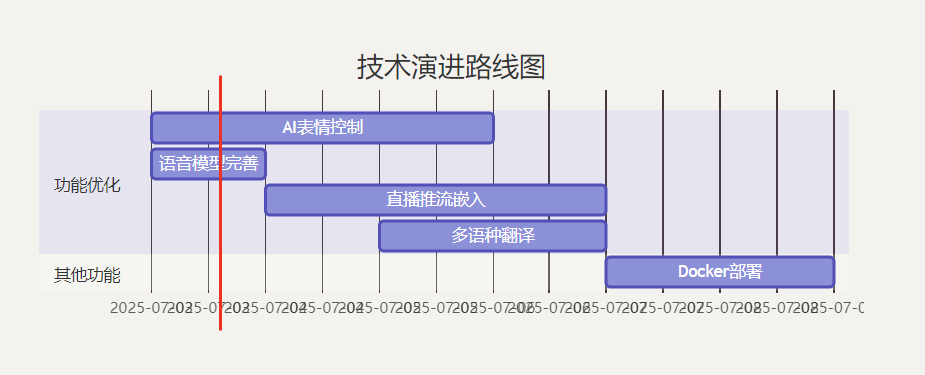
\includegraphics[width=\textwidth]{pic/gantt_roadmap.png}
%     \end{block}
%     \begin{alertblock}{关键里程碑}
%         \begin{itemize}
%             \item \textbf{2024 Q4}: 
%             \begin{itemize}
%                 \item 实现Wasm版FFmpeg,降低转码延迟30\%
%                 \item 部署GPT-SoVITS蒸馏模型 (<1GB内存)
%             \end{itemize}
%             \item \textbf{2025 Q1}:
%             \begin{itemize}
%                 \item 集成NeRF实现3D虚拟主播
%                 \item 支持LLM实时生成直播脚本
%             \end{itemize}
%         \end{itemize}
%     \end{alertblock}
% \end{frame}
% \begin{frame}{未来规划与技术展望}
%     \begin{columns}[T]
%         \begin{column}{0.5\textwidth}
%             \begin{exampleblock}{近期规划 (Next Steps)}
%                 \begin{itemize}
%                     \item \textbf{表情驱动升级}: \\
%                           引入AI模型,实现更智能、自然的 Live2D 表情自动控制。
%                     \item \textbf{语音功能扩展}: \\
%                           集成 Voice Conversion 技术,实现多语种实时翻译与声音克隆。
%                 \end{itemize}
%             \end{exampleblock}
%         \end{column}
%         \begin{column}{0.5\textwidth}
%             \begin{alertblock}{我们的最终目标}
%                 \Large
%                 打造一站式全自动下一代的AI虚拟直播平台!
%             \end{alertblock}
%         \end{column}
%     \end{columns}
% \end{frame}


\begin{frame}{我们的愿景}​
    \begin{center}​
        \Large 打造下一世代的一站式全自动AI虚拟直播平台​\\
    \end{center}​
    \vspace{0.5em}​
    \begin{center}​
        \large 由而使得机械的灵魂与人类的心脏同频共振​
    \end{center}​
\end{frame}

% --- Q&A页 --- 
% \begin{frame}
%     \centering
%     \Huge{\textbf{Q \& A}}
%     \vspace{2em}
%     \large{我们期待与各位深入探讨技术细节,\\共同推动AI直播技术的边界!}
%     \vspace{2em}
%     \Large{\textbf{感谢聆听}}
% \end{frame}


\begin{frame}{致谢}
    \begin{center}
        \huge 感谢您的聆听! \\
    \end{center}
    \begin{center} % 用center环境包裹图片,实现居中并排
        
\includegraphics[width=4cm]{pic/队伍徽标.jpg}
        \hspace{0.5cm} % 两个图片之间的水平间距,可按需调整
        
\includegraphics[width=4cm]{pic/项目图标.jpg}
    \end{center}
    \begin{center}
        \large 我们是DeepSleep项目团队, \\
        \large 期待与您一同探索AI领域的无垠边界!
    \end{center}
\end{frame}

\end{document}
